\chapter{Evaluation}
The last chapter of our thesis presents evaluation results, included in Attachment \ref{add:Outputs}, of all conducted experiments, described in detail in Chapter \ref{sec:medGenReportExperiments}, for the medical reports generation task. Each performed experiment was evaluated automatically with the common machine translation metrics. Furthermore, the outputs of the best models were manually evaluated by an experienced physician.

\section{Automatic evaluation}
First part of this chapter reports the results of the automatic evaluation of our trained models. An important thing to mention is that these metrics give us only an indication of which models could be theoretically performing well and not their true performance. Each image can be described in multiple different ways. The metrics only compare words between generated and reference texts with minimal logic to capture meaning. Therefore, they measure whether the texts are similar rather than having the same meaning. This fact is further intensified by the nature of our area, where we need to capture all findings appearing in the image and the overall diagnosis. \\

The evaluation was performed on a subset of 500 X-ray images. We subjected all models to standard automatic evaluation metrics used in image captioning and machine translation areas using NLG evaluation from \citet{sharma2017nlgeval}.

\subsection{Metrics}
This section outlines all NLG evaluation measured metrics applicable for the Czech language supplemented with the GLEU metric. For the embedding NLG evaluation metrics, the NLG package had to be modified in order to use Czech word2vec trained vectors from \citet{grave2018learning}.

\subsubsection*{BLEU}
BLEU metric has become a standard metric in the field of image captioning. It was first introduced in the \citet{papineni2002bleu} paper. This metric computes the number of common unigrams up to n-grams between the reference text and the generated one. Commonly used are unigrams up to tetragrams as they capture the similarities between texts the best. BLEU-4 thus uses unigrams up to tetragrams. The final BLEU score is the mean of the BLEU scores of all evaluated texts.

\subsubsection*{GLEU}
GLEU (Google BLEU) metric, presented in \citet{wu2016google}, is Google's alternative instead of BLEU for machine translation evaluation. For the sentence GLEU score, the n-gram precision and recall are calculated and the minimum of these values are taken as the results. All unigrams up to n-grams are taken for the calculation. The final corpus-level GLEU score is computed as the ratio of the sum of all matching n-grams and the sum of all n-grams used for precision or recall in the sentence-level case for all texts, instead of the mean of the sentence-level GLEU scores.

\subsubsection*{METEOR}
METEOR is a unigram-based F-score metric first defined in \citet{banerjee2005meteor}. In the beginning, it tries to match all unigrams from the generated text to zero or one unigram from the reference text. This could also include matching paraphrases, synonyms, stems, or others. The mapping with the minimum number of chunks is taken for subsequent calculation of precision and recall. The final score is the harmonic mean, where the recall is many times more significant than the precision, multiplied by a fragmentation penalty. In order to calculate this metric for Czech data, we had to modify the original NLG code and download the paraphrases for the Czech language.\footnote[1]{\url{https://github.com/cmu-mtlab/meteor/blob/master/data/paraphrase-cz.gz}}

\subsubsection*{ROUGE-L}
ROUGE-L metric, from \citet{lin2004rouge} paper, works with the word longest common subsequence (LCS) between the generated and reference text. The found subsequence does not have to be consecutive. The reasoning behind this metric is that longer common subsequences result in more similarities between the compared texts. ROUGE-L is an F-score metric and is therefore computed using both precision and recall based on the LCS.

\subsubsection*{CIDEr}
CIDEr\citep{vedantam2015cider} is another word-overlap metric. It first determines the TF-IDF weight vector representation of unigrams up to tetragrams for both texts. Thus for each generated and reference text, we obtain four vector representations. The cosine similarity is calculated for each of these vectors. The mean of these cosine similarities is then taken as the final score.

\subsubsection*{Embedding Average cosine similarity}
For both of the texts - generated and the reference, the embeddings of all words are averaged. The final score is then computed as the cosine similarity between these averaged embedding vectors.

\subsubsection*{Vector Extrema cosine similarity}
This metric was presented in \citet{forgues2014bootstrapping}. As in the previous case, it computes the cosine similarity between the generated and reference text. However, instead of the mean embeddings, the most extreme values (the largest in terms of absolute value) in each dimension are taken.

\subsubsection*{Greedy Matching score}
The final used metric is the Greedy Matching score from \citet{rus2012optimal}. For each word embedding in the generated text, the maximum cosine similarity is calculated against the words' embeddings of the reference text. These scores are then averaged by the total number of words in the generated text. The identical procedure is then used the other way round with the reference text. As the final score, the mean of these scores is taken.

\subsection{Results}
The results of the automatic evaluation are reported in Table \ref{tab01:AutoEvalBleu}, Table \ref{tab02:AutoEvalGleu}, and Table \ref{tab03:AutoEvalWordRest} for the standard NLP metrics and in Table \ref{tab04:AutoEvalEmbedding} for the embedding-based metrics. For metrics that are evaluated for different n-gram bases (BLEU and GLEU), we further refer to those working with up to tetragrams if not specified otherwise. Since there are no works solving our problem in the Czech language, we do not have a direct baseline to compare our results with and thus we will only compare them to each other.\\

For the BLEU and GLEU metrics, we can see in Tables \ref{tab01:AutoEvalBleu} and \ref{tab02:AutoEvalGleu} that the best results have the models, where the entire network was unfrozen during the training. This is naturally expected as the network has more space and freedom for learning. Moreover, the \textit{GEN-all-best}, with 0.0751 and 0.0928 for BLEU and GLEU respectively, surpassed the \textit{MED-all-best}, which utilized the medical GPT-2 model as the language model, by 0.3 on both BLEU and GLEU. The other \textit{best} models also show nice results and they are good candidates for further comparison. In general, the \textit{last} models are worse. The only exception is \textit{MED-dec-last}, where BLEU was higher than for the corresponding \textit{best} model. However, BLEU\textsubscript{1} - BLEU\textsubscript{3} are better for the \textit{MED-dec-best} model.\\ 

The same trend continues in the rest of the word-overlap metrics, presented in Table \ref{tab03:AutoEvalWordRest}. However, the \textit{MED-all-best} is worse than other \textit{best} models on most metrics. We can also notice that the \textit{MED-dec-last} surprisingly outperformed all models on CIDEr metric with 0.2978, whilst underperforming in others. The opposite phenomenon occurred for the \textit{MED-dec-best} model, which was the worst on CIDEr with 0.1798, but comparable to other \textit{best} models on the rest.\\

Regarding the embedding metrics evaluation listed in Table \ref{tab03:AutoEvalWordRest}, the \textit{GEN-dec-best} model beat the rest of the models, but the otherwise best \textit{GEN-all-best} model's results are very close to it. Surprisingly, the \textit{MED-dec-best} has better results on all of these metrics than the \textit{MED-all-best} model, where the whole model was trainable.\\

We can see that \textit{GEN-all-best}, which was trained on an entirely unfrozen network, model outperformed the other models in almost all metrics. Nevertheless, the model comes from the earlier phases of the training. All other \textit{best} models were performing well and outdid each other in different examined metrics. As we mentioned earlier, the automatic evaluation only suggests which models could be performing well, and their final performance will be determined by manual evaluation in the next section.

\begin{table}[h!]
\centering
\begin{tabular}{l@{\hspace{0.75cm}}D{.}{,}{0}D{.}{,}{1.2}D{.}{,}{2.3}D{.}{,}{2.3}D{.}{,}{2.3}D{.}{,}{2.3}}
\toprule
 & \mc{} & \mc{} & \mc{} & \mc{} & \mc{} & \mc{} \\
\pulrad{\textbf{Model}} & \mc{\pulrad{\textbf{Epoch}}} & \mc{\pulrad{\textbf{BLEU\textsubscript{1}}}} & \mc{\pulrad{\textbf{BLEU\textsubscript{2}}}} & \mc{\pulrad{\textbf{BLEU\textsubscript{3}}}} & \mc{\pulrad{\textbf{BLEU\textsubscript{4}}}} \\
\midrule
GEN-dec-best                & \mc{\phantom{0}28}            & \mc{0.2451}  & \mc{0.1489} & \mc{0.0951} & \mc{0.0655} \\
GEN-dec-last                 & \mc{100}            		 & \mc{0.2080}  & \mc{0.1207} & \mc{0.0764} & \mc{0.0519} \\
GEN-all-best                  & \mc{\phantom{0}13}            & \mc{0.2487}  & \mc{\textbf{0.1550}} & \mc{\textbf{0.1044}} & \mc{\textbf{0.0751}} \\
GEN-all-last                   & \mc{100}            		 & \mc{0.2161}  & \mc{0.1281} & \mc{0.0809} & \mc{0.0551} \\
MED-dec-best                & \mc{\phantom{0}13}            & \mc{\textbf{0.2526}}  & \mc{0.1511} & \mc{0.0951} & \mc{0.0617} \\
MED-dec-last                 & \mc{100}            		  & \mc{0.2207}  & \mc{0.1358} & \mc{0.0918} & \mc{0.0683} \\
MED-all-best                  & \mc{\phantom{0}76}            & \mc{0.2336}  & \mc{0.1447} & \mc{0.0987} & \mc{0.0726} \\
MED-all-last                   & \mc{100}            		  & \mc{0.2145}  & \mc{0.1322} & \mc{0.0877} & \mc{0.0630} \\
\bottomrule
\multicolumn{6}{l}{\footnotesize \textit{Note:} All values are rounded to 4 decimal places.}
\end{tabular}

\caption{BLEU evaluation results comparison.}\label{tab01:AutoEvalBleu}
Models are described in Chapter \ref{sec:medGenReportExperiments},
\textit{best} suffix denotes the best trained models, \textit{last} denotes the last trained models, BLEU\textsubscript{n} index states the number of n-grams used
\end{table}

\begin{table}[h!]
\centering
\begin{tabular}{l@{\hspace{0.75cm}}D{.}{,}{0}D{.}{,}{1.2}D{.}{,}{2.3}D{.}{,}{2.3}D{.}{,}{2.3}D{.}{,}{2.3}}
\toprule
 & \mc{} & \mc{} & \mc{} & \mc{} & \mc{} & \mc{} \\
\pulrad{\textbf{Model}} & \mc{\pulrad{\textbf{Epoch}}} & \mc{\pulrad{\textbf{GLEU\textsubscript{1}}}} & \mc{\pulrad{\textbf{GLEU\textsubscript{2}}}} & \mc{\pulrad{\textbf{GLEU\textsubscript{3}}}} & \mc{\pulrad{\textbf{GLEU\textsubscript{4}}}} \\
\midrule
GEN-dec-best                & \mc{\phantom{0}28}            & \mc{0.2122}  & \mc{0.1460} & \mc{0.1094} & \mc{0.0875} \\
GEN-dec-last                 & \mc{100}            		 & \mc{0.1900}  & \mc{0.1275} & \mc{0.0951} & \mc{0.0758} \\
GEN-all-best                  & \mc{\phantom{0}13}            & \mc{0.2154}  & \mc{\textbf{0.1502}} & \mc{\textbf{0.1146}} & \mc{\textbf{0.0928}} \\
GEN-all-last                   & \mc{100}            		 & \mc{0.1902}  & \mc{0.1290} & \mc{0.0962} & \mc{0.0767} \\
MED-dec-best                & \mc{\phantom{0}13}            & \mc{\textbf{0.2170}}  & \mc{0.1480} & \mc{0.1104} & \mc{0.0873} \\
MED-dec-last                 & \mc{100}            		 & \mc{0.1966}  & \mc{0.1360} & \mc{0.1038} & \mc{0.0848} \\
MED-all-best                  & \mc{\phantom{0}76}           & \mc{0.2083}  & \mc{0.1447} & \mc{0.1108} & \mc{0.0903} \\
MED-all-last                   & \mc{100}            		 & \mc{0.1968}  & \mc{0.1362} & \mc{0.1033} & \mc{0.0835} \\
\bottomrule
\multicolumn{5}{l}{\footnotesize \textit{Note:} All values are rounded to 4 decimal places.}
\end{tabular}

\caption{GLEU evaluation results comparison.}\label{tab02:AutoEvalGleu}
Models are described in Chapter \ref{sec:medGenReportExperiments},
\textit{best} suffix denotes the best trained models, \textit{last} denotes the last trained models, GLEU\textsubscript{n} index states the number of n-grams used
\end{table}

\begin{table}[h!]
\centering
\begin{tabular}{l@{\hspace{0.75cm}}D{.}{,}{0}D{.}{,}{1.2}D{.}{,}{2.3}D{.}{,}{2.3}D{.}{,}{2.3}D{.}{,}{2.3}}
\toprule
 & \mc{} & \mc{} & \mc{} & \mc{} & \mc{} & \mc{} \\
\pulrad{\textbf{Model}} & \mc{\pulrad{\textbf{Epoch}}} & \mc{\pulrad{\textbf{METEOR}}} & \mc{\pulrad{\textbf{ROUGE-L}}} & \mc{\pulrad{\textbf{CIDEr}}} \\
\midrule
GEN-dec-best                & \mc{\phantom{0}28}            & \mc{0.1103}  & \mc{0.2087} & \mc{0.2290} \\
GEN-dec-last                 & \mc{100}           			 & \mc{0.0952}  & \mc{0.1878} & \mc{0.2038} \\
GEN-all-best                  & \mc{\phantom{0}13}            & \mc{\textbf{0.1138}}  & \mc{\textbf{0.2125}} & \mc{0.2964} \\
GEN-all-last                   & \mc{100}            		 & \mc{0.0988}  & \mc{0.1958} & \mc{0.2240} \\
MED-dec-best                & \mc{\phantom{0}13}            & \mc{0.1133}  & \mc{0.2074} & \mc{0.1798} \\
MED-dec-last                 & \mc{100}            		  & \mc{0.1013}  & \mc{0.1953} & \mc{\textbf{0.2978}} \\
MED-all-best                  & \mc{\phantom{0}76}            & \mc{0.1072}  & \mc{0.2027} & \mc{0.2658} \\
MED-all-last                   & \mc{100}            		  & \mc{0.1003}  & \mc{0.1988} & \mc{0.2598} \\
\bottomrule
\multicolumn{5}{l}{\footnotesize \textit{Note:} All values are rounded to 4 decimal places.}
\end{tabular}

\caption{Word-overlap metrics evaluation results.}\label{tab03:AutoEvalWordRest}
Models are described in Chapter \ref{sec:medGenReportExperiments},
\textit{best} suffix denotes the best trained models, \textit{last} denotes the last trained models
\end{table}

\begin{table}[h!]

\centering
\begin{tabular}{l@{\hspace{0cm}}D{.}{,}{0}D{.}{,}{1.2}D{.}{,}{2.3}D{.}{,}{2.3}D{.}{,}{2.3}D{.}{,}{2.3}}
\toprule
 & \mc{} & \mc{} & \mc{} & \mc{} & \mc{} \\
\pulrad{\textbf{Model}} & \mc{\pulrad{\textbf{Epoch}}} & \mc{\pulrad{\textbf{\parbox{2.35cm}{\centering Embedding \\ Average}}}} & \mc{\pulrad{\textbf{\parbox{1.775cm}{\centering Vector \\ Extrema}}}} & \mc{\pulrad{\textbf{\parbox{1.95cm}{\centering Greedy \\ Matching}}}} \\
\midrule
GEN-dec-best                & \mc{\phantom{0}28}             & \mc{\textbf{0.8023}} & \mc{\textbf{0.4092}} & \mc{\textbf{0.6340}} \\
GEN-dec-last                 & \mc{100}           			  & \mc{0.7778} & \mc{0.3765} & \mc{0.6169} \\
GEN-all-best                  & \mc{\phantom{0}13}             & \mc{0.7974} & \mc{0.4050} & \mc{0.6327} \\
GEN-all-last                   & \mc{100}           			  & \mc{0.7854} & \mc{0.3950} & \mc{0.6192} \\
MED-dec-best                & \mc{\phantom{0}13}             & \mc{0.7998} & \mc{0.4089} & \mc{0.6265} \\
MED-dec-last                 & \mc{100}          			  & \mc{0.7758} & \mc{0.3738} & \mc{0.6160} \\
MED-all-best                  & \mc{\phantom{0}76}            & \mc{0.7902} & \mc{0.4019} & \mc{0.6241} \\
MED-all-last                   & \mc{100}          			  & \mc{0.7754} & \mc{0.3796} & \mc{0.6175} \\
\bottomrule
\multicolumn{6}{l}{\footnotesize \textit{Note:} All values are rounded to 4 decimal places.}
\end{tabular}

\caption{Embedding metrics evaluation results.}\label{tab04:AutoEvalEmbedding}
Models are described in Chapter \ref{sec:medGenReportExperiments},
\textit{best} suffix denotes the best trained models, \textit{last} denotes the last trained models
\end{table}

\newpage
\section{Manual evaluation}
This section presents the results of the manual evaluation. We would like to express our gratitude to MUDr.\ Martin Hyršl from the University Hospital Hradec Králové for the execution of manual evaluation on our generated reports. The manual evaluation was performed on a total of 40 X-ray images and their corresponding reports for all four \textit{best} models from the previous section. The X-rays are divided into two equally sized groups for evaluation - with and without the presence of any medical findings.

\subsection{Method}
All images with the presence of any disease were evaluated using the following method. Each report is assigned at least one of three non-disjunctive categories. The first category (Accurate Finding) reflects the cases where the report contains at least one correct finding or diagnosis. The next category (Missing Finding) describes cases where an important part of the diagnosis is missing from the report. In the last category (Incorrect Finding) fall reports that contain untrue facts. In addition, we also report the number of completely accurate reports. We chose this method over the one in the original paper as it has greater informational value.\\

The images of healthy patients were classified into two cases only according to whether they contained any finding or not.

\subsection{Results}
The obtained results of the manual evaluation are shown in Table \ref{tab05:ManualEvalFinding} and Table \ref{tab06:ManualEvalNormal}. In the previous section, we concluded that all \textit{best} models are comparable, with \textit{GEN-all-best} being the best. Nevertheless, we can clearly see in the results that the  \textit{MED} models perform overall better than the \textit{GEN} models. In cases where any disease is present, the \textit{MED-all-best} found some correct finding in more cases than any other model, while maintaining comparable values in the rest of the categories. From the other side, the \textit{MED-dec-best} model made the least number of mistakes, 50\% less than the \textit{GEN-dec-best} model, and found any right finding as many times as the \textit{GEN-dec-best}. In terms of completely accurate predictions, the \textit{MED} models also turned out better.\\

On the images without any anomaly, the results of all models are very similar and they generally predict a small number of false positives. However, the results of two models stand out - the \textit{MED} models. In particular, the \textit{MED-all-best} made more mistakes than the others and \textit{MED-dec-best} made the least in contrast. This result is in correspondence with the evaluation on the images where problems occur. The \textit{MED-all-best} is \qq{more courageous} and tries to find something. On the other hand, the \textit{MED-dec-best} model is \qq{more cautious} and rather assumes that the patient is healthy. In overall, the \textit{MED-all-best} seems to be optimized for Recall (high \textit{AF}), while the \textit{MED-dec-best} for Precision (low \textit{IF}).\\

After a discussion, the physician did not rate the final generated reports as very beneficial due to the following reasons. Firstly, in the medical environment, it is critical to find all the true pathologies on the X-ray image and no others for the purposes of proper treatment. Moreover, he also mentioned that it would be better to have a more structured form of the reports and not describe the normal conditions so much. Lastly, he mentioned the slightly lower quality of the translations.\\

Nevertheless, we see the final result in a positive way. In our opinion, the prediction works reasonably well. Although the model rarely provides a completely accurate corresponding report, it identifies at least one correct finding in almost half of the cases. Furthermore, healthy radiographs are described as normal in the majority of cases. Taking everything into account, it is clear that the models are not ready for deployment in the hospitals, however, we consider the overall outcome as promising results.

\begin{table}[h!]
\centering
\begin{tabular}{l@{\hspace{0.75cm}}D{.}{,}{5.0}D{.}{,}{5.0}D{.}{,}{5.0}D{.}{,}{5.0}D{.}{,}{5.0}D{.}{,}{5.0}}
\toprule
 & \mc{} & \mc{} & \mc{} & \mc{} \\
\pulrad{\textbf{Model}} & \mc{\pulrad{\textbf{AF (\#/\%)}}} & \mc{\pulrad{\textbf{MF (\#/\%)}}} & \mc{\pulrad{\textbf{IF (\#/\%)}}} & \mc{\pulrad{\textbf{CA (\#/\%)}}} \\
\midrule
GEN-dec-best      & \mc{7 (35\%)}  & \mc{18 (90\%)}  & \mc{12 (60\%)}                      & \mc{1 (\phantom{0}5\%)} \\
GEN-all-best        & \mc{5 (25\%)}  & \mc{18 (90\%)}  & \mc{\phantom{0}8 (40\%)}     & \mc{1 (\phantom{0}5\%)} \\
MED-dec-best	 & \mc{7 (35\%)}  & \mc{18 (90\%)}  & \mc{\phantom{0}6 (30\%)}      & \mc{2 (10\%)} \\
MED-all-best       & \mc{9 (45\%)}  & \mc{17 (85\%)}  & \mc{\phantom{0}8 (40\%)}      & \mc{2 (10\%)} \\
\bottomrule
\end{tabular}

\caption{Manual evaluation results - with findings.}\label{tab05:ManualEvalFinding}
Evaluation categories are described above, \textit{AF} - Accurate Finding, \textit{MF} - Missing Finding, \textit{IF} - Incorrect Finding, \textit{CA} - Completely Accurate
\end{table}


\begin{table}[h!]
\centering
\begin{tabular}{l@{\hspace{0.75cm}}D{.}{,}{5.0}D{.}{,}{5.0}D{.}{,}{5.0}D{.}{,}{5.0}}
\toprule
 & \mc{} & \mc{} & \mc{} & \mc{} \\
\pulrad{\textbf{Model}} & \mc{\pulrad{\textbf{NF (\#/\%)}}} & \mc{\pulrad{\textbf{IF (\#/\%)}}} \\
\midrule
GEN-dec-best      & \mc{17 (85\%)}   & \mc{3 (15\%)} \\
GEN-all-best        & \mc{17 (85\%)}   & \mc{3 (15\%)} \\
MED-dec-best	 & \mc{19 (95\%)}   & \mc{1 (\phantom{0}5\%)} \\
MED-all-best       & \mc{16 (80\%)}   & \mc{4 (20\%)} \\
\bottomrule
\end{tabular}

\caption{Manual evaluation results - without findings.}\label{tab06:ManualEvalNormal}
Evaluation categories are described above, \textit{NF} - No Finding, \textit{IF} - Incorrect Finding
\end{table}

\newpage
\section{Examples}
In the previous section, we evaluated all trained models and determined their actual performance. Illustrations of generated outputs in a variety of cases are depicted in Figure~\ref{fig01:Examples1} and Figure~\ref{fig02:Examples2} for the best performing models. In almost all cases, as reported in the manual evaluation results above, there is at least one matching finding in the generated report. \\

Another observation is that the models tend to describe a lot of irrelevant information on the X-ray image that describes normal conditions. Again, this is based on the underlying data, as the vast majority of reports contain this kind of description.\\

We can notice, that in some cases both the translation and the generated outputs contain some grammatical or syntactic issues. This is a consequence of the automatic machine translation noise. The original data are already noisy, as they contain some undesirable elements replacing sensitive patient data, which is further intensified by the machine translation process. Moreover, these elements are removed from the sentences during training, sometimes resulting in an incoherent part of the text.

\begin{figure}[h]\centering
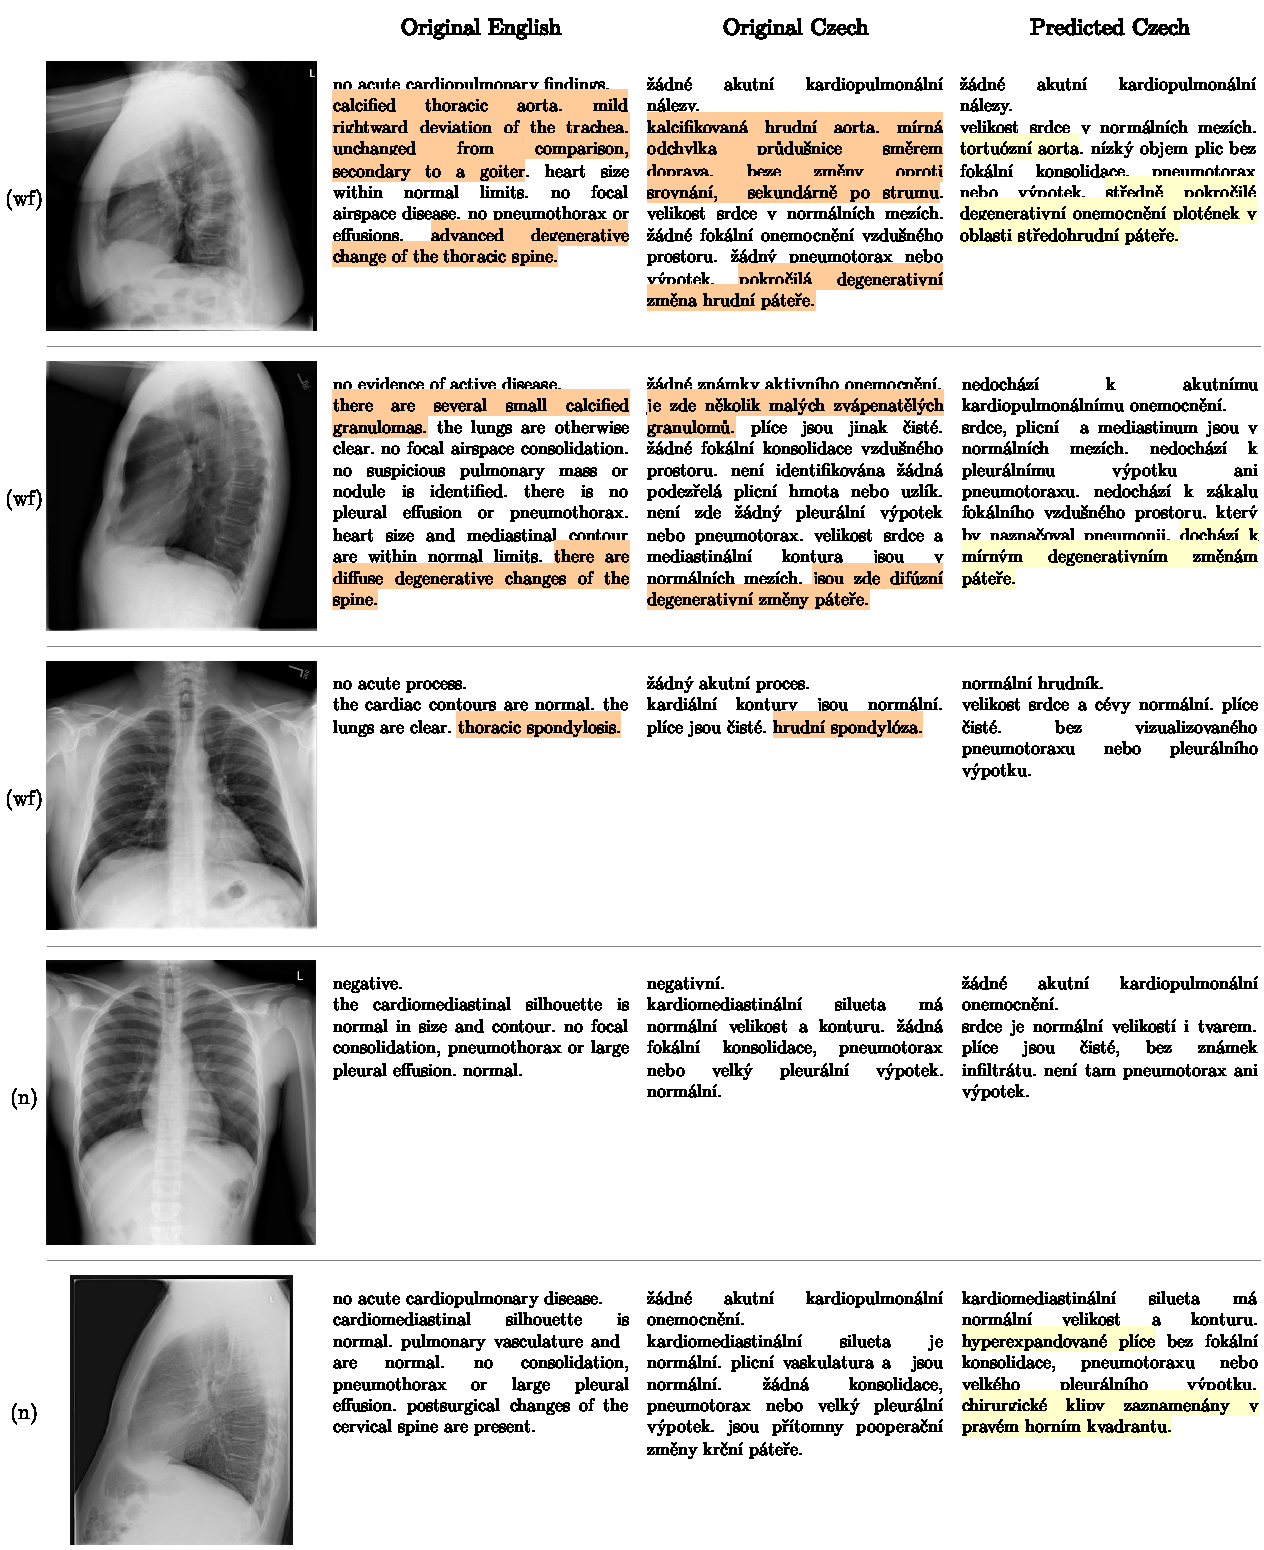
\includegraphics[width=145mm, height=177.5mm]{../img/Examples1}
\caption{Examples of generated reports by the \textit{MED-all-best} model.}
\label{fig01:Examples1}
\textit{wf} denotes X-ray images with some finding, \textit{n} denotes normal X-ray images\\
Highlighted parts of the text indicate findings\\
Prediction categories:
\textbf{1} - \textit{AF}, \textit{CA};
\textbf{2} - \textit{AF}, \textit{MF};
\textbf{3} - \textit{MF};
\textbf{4} - \textit{NF};
\textbf{5} - \textit{IF}
\end{figure}

\begin{figure}[h]\centering
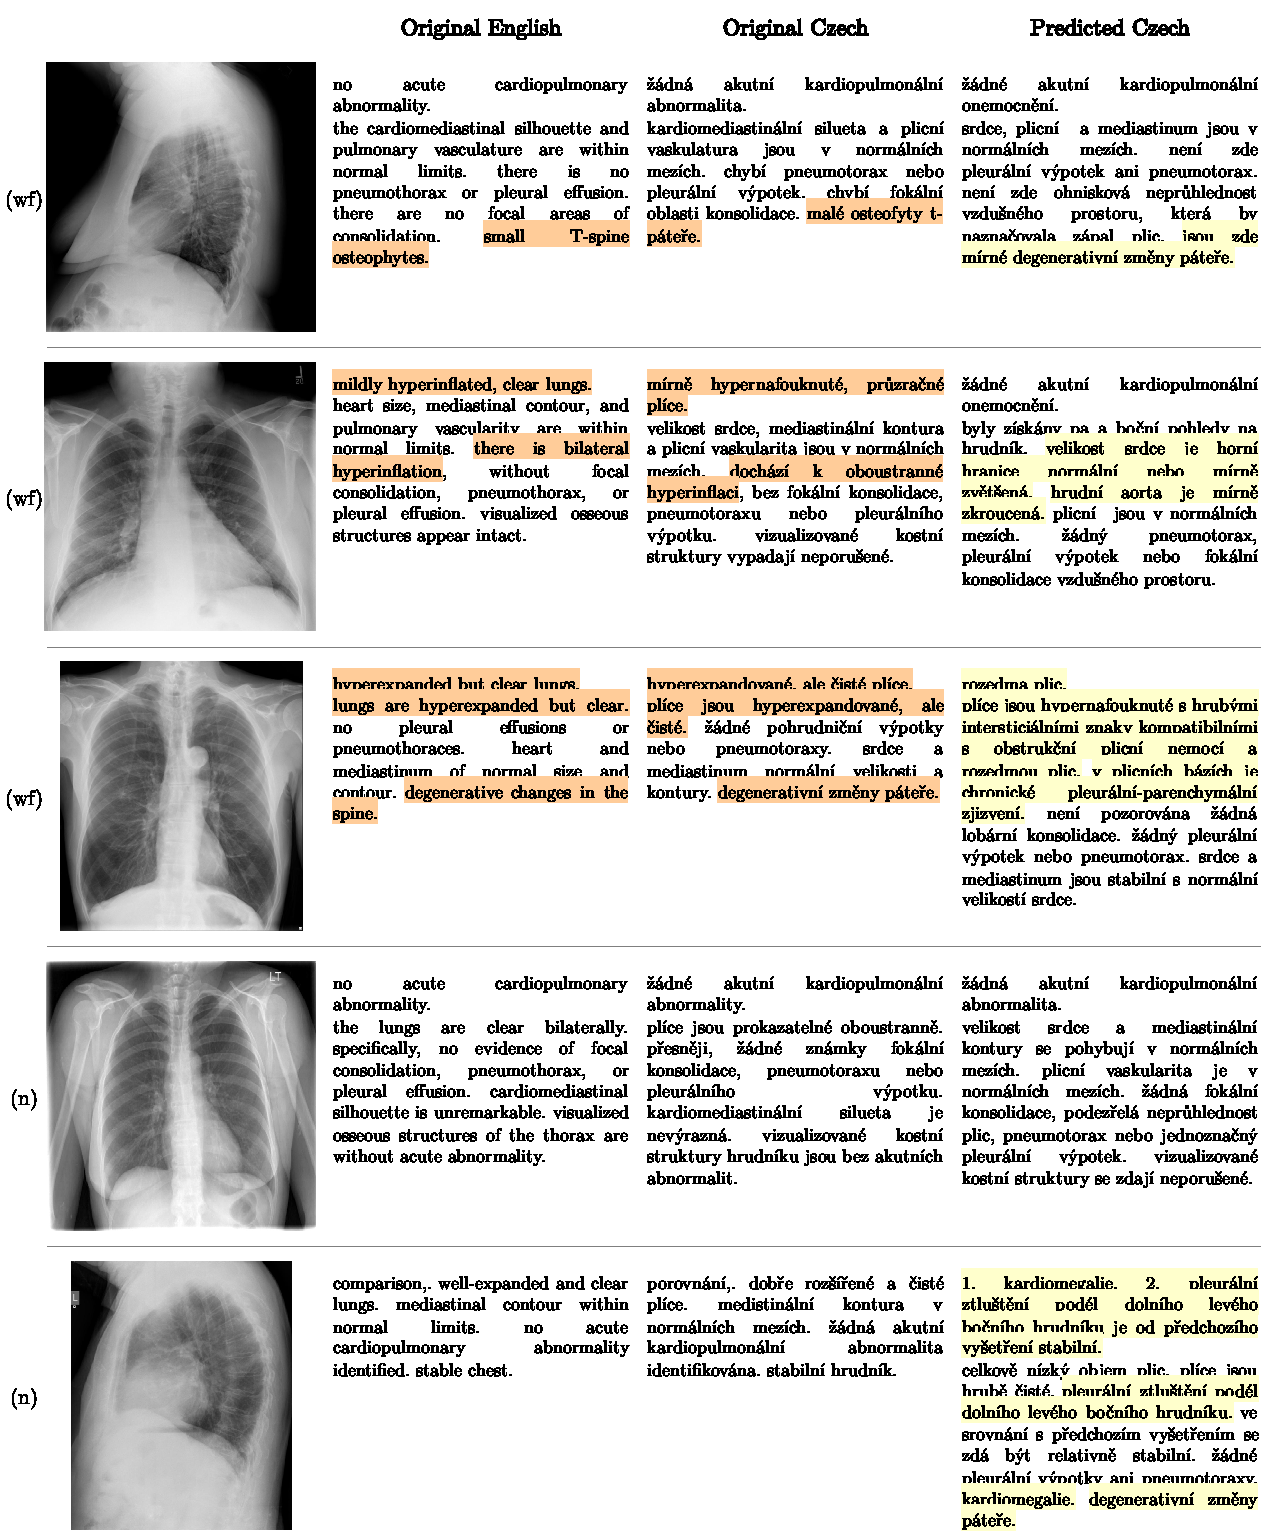
\includegraphics[width=145mm, height=177.5mm]{../img/Examples2}
\caption{Examples of generated reports by the \textit{MED-dec-best} model.}
\label{fig02:Examples2}
\textit{wf} denotes X-ray images with some finding, \textit{n} denotes normal X-ray images\\
Highlighted parts of the text indicate findings\\
Prediction categories:
\textbf{1} - \textit{AF}, \textit{CA};
\textbf{2} - \textit{MF}, \textit{IF};
\textbf{3} - \textit{AF}, \textit{MF};
\textbf{4} - \textit{NF};
\textbf{5} - \textit{IF}
\end{figure}

\newpage
\section{Conclusion}
We have evaluated our models in several different ways. The automatic evaluation was comprised of many NLP metrics that provided us with basic information about the models and have given us an idea of their performance. Nevertheless, these hypotheses had to be verified by manual evaluation, as the automatic metrics are very sensitive, especially in the medical environment, where a diagnosis can be written in multiple different ways. Finally, the manual evaluation has given us the true performance of all our \textit{best} models. We have found that the model, which came out best overall in the automatic evaluation, and generally both \textit{GEN} models, were outperformed by the \textit{MED} models. From the overall results, we have come to the conclusion that fine-tuning the Czech GPT-2 on medical data helps the final performance.





